\chapter{Tools}

\section{Internal}
\subsection{cfstool}
\subsection{cplreader}

\section{Pre-Processors}
\subsection{ANSYS}

\begin{enumerate}
   \item{Document mkmesh/mkhdf5
       \attachfile[icon=PushPin,description={ANSYS mkmesh and mkhdf5 extension.},mimetype=text/plain]{attachments/mkmesh.mlib.txt}
       \attachfile[icon=PushPin,description={ANSYS mkmesh AWK script.},mimetype=text/plain]{attachments/mkmesh.txt}
     }
   \item{How to modify third party ANSYS /prep7 meshes to write them with mkhdf5
       \attachfile[icon=PushPin,description={Result of File -> Export -> ANSYS in ICEM CFD.},mimetype=text/plain]{attachments/Pfeifenfussmodell_modificated_swept.in.txt}
       \attachfile[icon=PushPin,description={ANSYS input script for converting ICEM mesh to mkhdf5 mesh.},mimetype=text/plain]{attachments/icem_to_ansys.in.txt}
     }
\end{enumerate}



\subsection{GiD}
\subsubsection{GiD im Batchmodus}

\noindent Wie ruf ich denn ein nacs gid script von der kommandozeile auf?

\begin{enumerate}
   \item{Erzeuge ein TCL-File example.bch (Endung bch wichtig) mit folgendem Inhalt: \input{pygmentized/gid_batch}}
   \item{Starte dann GiD mittels: {\tt gid -p NACS -n2 -b example.bch}}
\end{enumerate}

\noindent und los gehts! Sollte  irgendwas nicht funktionieren, dann kannst Du
erst mal einen Blick in das batch file werfen:

\noindent Utilities $\rightarrow$ Tools $\rightarrow$ Read Batch Window ...

\noindent und dann mittels des File  Dialoges das Batch File auswählen und mit
dem Button See File... den Inhalt anzeigen lassen

\paragraph{GiD Passwortserver auf rom}
\begin{itemize}
\item{Alle wichtigen Lizenzinformationen liegen auf rom:/usr/local/passerver/lic\_info\_rom.txt}
\item{Eine Anleitung zur Installation des Passwortservers liegt in rom:/usr/local/passerver/gidlicinst.pdf }
\item{Port 7073 in der Firewall freischalten}
\item{Folgendes Shellscript nach /etc/init.d/gidpasserver speichern:
  \input{pygmentized/gid_pw_server}
  \attachfile[icon=PushPin,description={openSUSE Init script for GiD license server.},mimetype=text/plain]{attachments/gid_pw_server.txt}
}
\item{Skript in den Bootprozess aufnehmen mit: {\tt insserv /etc/init.d/gidpasserver} }
\end{itemize}


\subsection{Gmsh}

GMSH \cite{Geuzaine2009,GmshWebSite} (simple  Meshes erzeugen, einziges Format
ausser HDF5  und GMV (auch UNV), das  CFS++ sowohl lesen (HDF5  Gitter und Daten,
GMV: Gitter, GMSH: Gitter) als  auch schreiben (HDF5,GMV,GMSH Gitter und Daten und
Named Enitities)  kann), Vorteil: Absolut  frei verfügbar für  Windows, Linux,
Mac (ANSYS und GiD sind alles andere als frei)

\begin{table}[tb]
\centering
\begin{minipage}{18cc}\caption{Gmsh Tutorials}
\label{tab:tablelabel}
\end{minipage}
\par\medskip\noindent
\begin{tabular}{ll}
  \toprule
  {\bf Tutorial} & {\bf URL} \\ \otoprule
  Meshgenerierung für Dolfyn & \url{http://www.dolfyn.net/dolfyn/gmsh/tutorial00.html} \\
  AMCG Tutorial & \url{http://amcg.ese.ic.ac.uk/ index.php?title=Local:Gmsh_tutorial} \\
  Introduction to Gmsh & \url{http://perso.uclouvain.be/vincent.legat/ teaching/documents/meca2170-jfr-notes-v1.0.pdf} \\
  Gmsh screencasts & \url{http://www.geuz.org/gmsh/screencasts/} \\
  Meshgenerierung für TiberCAD & \url{http://www.tibercad.org/documentation/ tutorial/list} \\
  Gmsh GUI Tutorial I & \url{http://ffep.sourceforge.net/Download/ gui\_tutorial.pdf}\\
  Gmsh GUI Tutorial II & \url{http://www.geuz.org/gmsh/doc/gui\_tutorial\_2/ gui\_tutorial\_2.pdf}\\
  Demo Gmsh - Step import - Msh export & \url{http://vimeo.com/3287369}\\
  \bottomrule
\end{tabular} 
\end{table}

The  Gmsh scripting language  shares the  same syntax  with the  C programming
language. Here we present a simple example where every geometrical entity will
be mapped  to exactly  one finite  element.  This is  achieved by  setting the
characteristic length  of the geometry nodes  to a value larger  than the edge
length of the geometrical entities.  The grid achieved therewith has been used
to test the crosspoint identification code.

\input{pygmentized/gmsh_cp_test}
\attachfile[icon=PushPin,description={Gmsh input script for crosspoint mesh.},mimetype=text/plain]{attachments/gmsh_cp_test.txt}

\begin{figure}[htb] 
  \centering
  \begin{overpic}[width=0.4\textwidth]{pics/gmsh_cp_test}
%    \put(10,20){\textcolor{white}{\bf The electrostatic man!}}
  \end{overpic}
  \caption{Crosspoint test geometry in Gmsh}
  \label{fig:gmsh_cp_test}
\end{figure}%
%

The script presented here just generates the geometry. The Meshing needs to be
done  by switching  to  {\it Mesh}  mode in  the  GUI and  then clicking  {\it
2D}.  This will  generate a  mesh of  first order  elements. To  get quadratic
elements one needs  to click on {\it Second order}.  Afterwards one just needs
to click on {\it Save} or {\it File} $\rightarrow$ {\it Save Mesh}.

The same thing may be achieved from the command line using the following command:
\begin{verbatim}
gmsh -2 -o output.msh -format msh2 -bin -nopopup -noview input.geo
\end{verbatim}

It  is  very important  to  assign the  elements  to  physical entities  ({\tt
Physical Surface}  or {\tt Physical Volume}). Otherwise  elements of different
dimensions  (e.g. triangles  and tetras)  may end  up in  the same  region for
CFS++.  In such a  case CFS++  will obviously  complain! The  textual argument
given to  {\tt Physical Surface} or  {\tt Physical Volume} will  be the region
name for CFS++.

\noindent Creating a mesh from an image:
\input{pygmentized/gmsh_mesh_from_pic}
\attachfile[icon=PushPin,description={Gmsh input script for generating a mesh from an image.},mimetype=text/plain]{attachments/gmsh_mesh_from_pic.txt}

\newpage

\section{Post-Processors}

\subsection{ANSYS}

The main source  of documentation for post-processing in  ANSYS Classic is the
{\it  Basic Analysis  Guide -  Chapter 5.  The General  Postprocessor (POST1)}
which can be  found in the ANSYS online help.  A modelling and post-processing
guide               can               also              be               found
here\footnote{\url{http://www-old.hallf.kth.se/\~mart/Demo\_Ansys\_classic.pdf}}.
One  Example  in CADFEM  Service  Newsletter  6/2003 (Ergebnisbeurteilung  bei
symmetrischen
Modellen)\footnote{\url{http://www.cadfem.at/fileadmin/files/9\_service\_newsletter/2003/0306/Newsletter\_06\_2003.pdf}}

The mapping  from CFS++ result  types to ANSYS  results is done in  the method
{\tt    void    AnsysBinlibIfaceGeneral::MapInternal2ANSYSNodeDof(SolutionType
solType)}                    in                    the                    file
{\tt source/DataInOut/SimInOut/AnsysRST/AnsysBinlibIfaceGeneral.cc}.

\textcolor{red}{ATTENTION:  It has  been found,  that there  exists  a problem
whenever the grid from CFS++ contains quadratic pyramid elements. This problem
manifests itself  as a  segfault of  ANSYS Classic. The  same input  file does
however not cause  a problem for the CFX post-processor.  This behavior can be
reproduced by the test suite case {\tt TESTSUIT/cfstool/hdf5\_to\_rst}, where the {\tt
.rst} file {\tt results\_rst/refelems\_ms1.rst} exhibits this behavior.}

Plot    nodal   solution   elecPot    on   .rst    from   test    suite   case
{\tt CFS\_TESTSUITE/TESTSUIT/cfstool/ hdf5\_to\_rst/results\_rst}

\begin{verbatim}
/POST1  
INRES,ALL   
FILE,'output_ms1','rst','.' 
SET,FIRST   
plnsol,volt
\end{verbatim}%
%
Postprocessing  can also  be accessed  via the  ANSYS Main  Menu $\rightarrow$
General  Postproc $\rightarrow$  Results Viewer  $\rightarrow$  Select Results
File  $\rightarrow$   Choose  a  result  item   $\rightarrow$  Nodal  Solution
$\rightarrow$ DOF Solution $\rightarrow$ Electric Potential $\rightarrow$ Plot
Results Button (left-most colorful one)

For plotting element results use the {\tt plesol} command.

\begin{figure}[htb]
  \centering
  \begin{overpic}[grid,tics=10,width=0.5\textwidth]{pics/ansys}
    \put(10,20){\textcolor{white}{\bf The electrostatic man!}}
  \end{overpic}
  \caption{Postprocessing the electrostatic man with ANSYS Classic}
  \label{fig:ansys}
\end{figure}%

The plot in Fig. \ref{fig:ansys} has been generated by the following commands\footnote{\url{http://www.mece.ualberta.ca/tutorials/ansys/PP/Slice/Slice.html}}:

\begin{verbatim}
/POST1  
INRES,ALL   
FILE,'man_model_ms1','rst','.' 
SET,FIRST
wpoffs,,,-0.3
/type,,8
/cplane,1
plnsol,volt
\end{verbatim}%
%
To show elements colored by region and the according region number (which is encoded as material MAT in .rst) and afterwards select the elements with MAT=4 the following sequence of commands may be used (cf. Fig. \ref{fig:ansys_eplo_mat}):
%
\begin{verbatim}
/POST1  
INRES,ALL   
FILE,'chargeaxi_ms1','rst','.' 
SET,FIRST
/PNUM,MAT,1
eplo
esel,s,mat,,4
elist
\end{verbatim}%
%
\begin{figure}[htb] 
  \centering
  \begin{overpic}[width=0.5\textwidth]{pics/ansys_eplo_mat}
%    \put(10,20){\textcolor{white}{\bf The electrostatic man!}}
  \end{overpic}
  \caption{Element plot with material numbers}
  \label{fig:ansys_eplo_mat}
\end{figure}%

To get information about available result sets, one can write the following sequence of commands
%
\begin{verbatim}
/POST1  
INRES,ALL   
FILE,'pml3d_ms1','rst','.' 
SET,list,2
\end{verbatim}%
%
which will produce the following output
%
\begin{verbatim}
  *****  INDEX OF DATA SETS ON RESULTS FILE  *****

   SET   TIME/FREQ    LOAD STEP   SUBSTEP  CUMULATIVE
     1  119.37             1         1         1
    pml3d step: 1, frequency: 119.366, real                                 

     2  119.37             1         1         1 (IMAGINARY)
    pml3d step: 1, frequency: 119.366, imag
\end{verbatim}%
%
Therefore to display the imaginary part of the solution the following sequence
of commands can be used (cf. Fig. \ref{fig:ansys_pml3d})
%
\begin{verbatim}
% Select imaginary part of first load step
set,1,,,1
plnsol,pres
% Select real part of first load step
set,1,,,0
plnsol,pres
\end{verbatim}%
%
Whether the  real/imag parts or  the abs/phase parts  of a complex  result are
saved in  the {\tt .rst} file depends  on the settings made  in the simulation
{\tt .xml} file.

\begin{figure}[htb] 
  \centering 
  \subfloat[Real part.]{
    \label{fig:ansys_pml3d_real}
    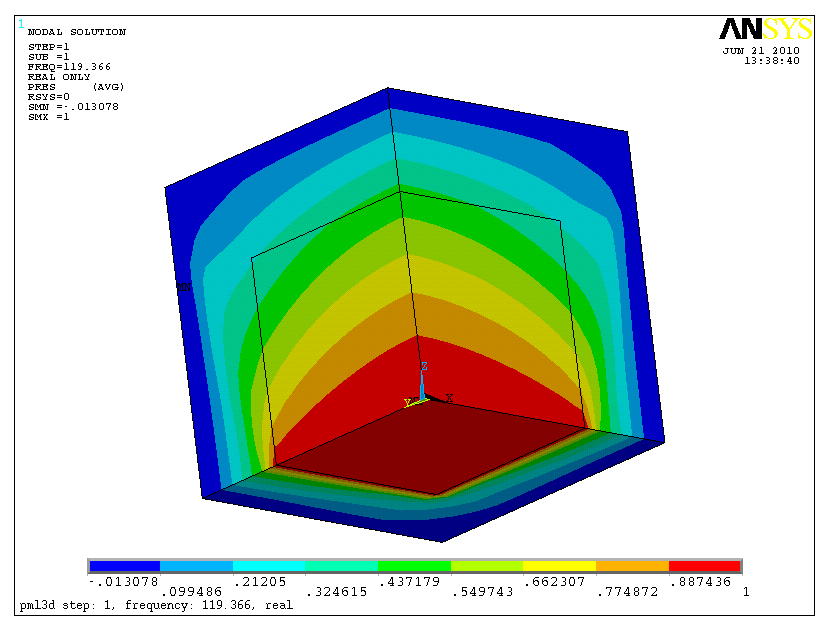
\includegraphics[width=6cm]{pics/ansys_pml3d_real} }
  \qquad
  \subfloat[Imaginary part.]{
    \label{fig:ansys_pml3d_imag}
    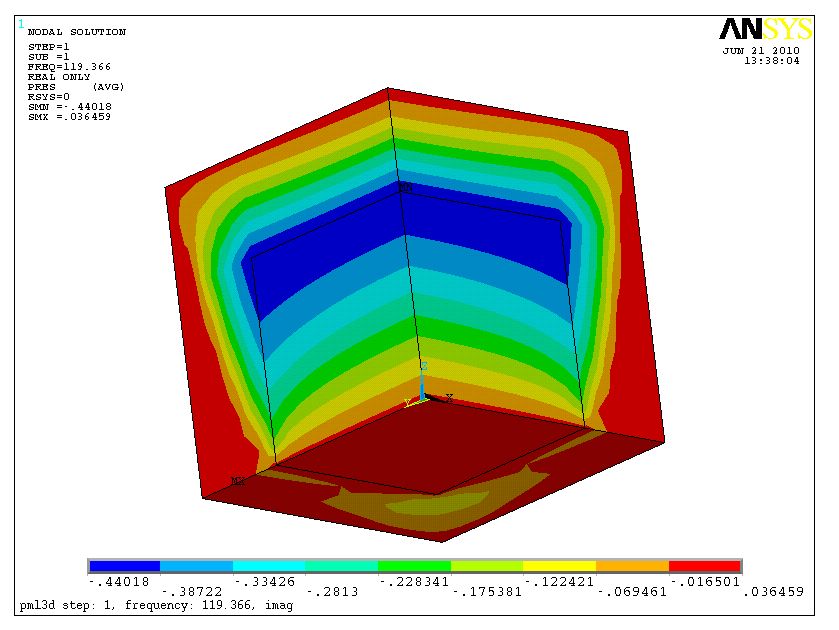
\includegraphics[width=6cm]{pics/ansys_pml3d_imag}
  } 
  \caption{Contour plots of acoustic pressure for acoustic pml3d testsuite example.}
  \label{fig:ansys_pml3d}
\end{figure}

While debugging the  ANSYS {\tt .rst} output writer it  was often necessary to
dump the {\tt .rst} file within ANSYS. This can be achieved using the follwing
sequence of commands.
%
\begin{verbatim}
/AUX2   
FORM,LONG   
FILEAUX2,'chargeaxi_ms1','rst',' '  
DUMP,ALL
\end{verbatim}
%
In the ANSYS GUI the same  functionality can be reached via File $\rightarrow$
List $\rightarrow$ Binary Files...

\newpage
\subsection{GiD}

\begin{figure}[htb] 
  \centering
  \begin{overpic}[grid,tics=10,width=0.5\textwidth]{pics/gid}
    \put(10,20){\textcolor{white}{\bf The electrostatic man!}}
  \end{overpic}
  \caption{Postprocessing the electrostatic man with GiD}
  \label{fig:gid}
\end{figure}%

\newpage
\subsection{Gmsh}

\begin{figure}[htb] 
  \centering
  \begin{overpic}[grid,tics=10,width=0.3\textwidth]{pics/gmsh}
    \put(10,20){\textcolor{white}{\bf The electrostatic man!}}
  \end{overpic}
  \caption{Postprocessing the electrostatic man with Gmsh}
  \label{fig:gmsh}
\end{figure}%
%
Postprocessing in  Gmsh is  mainly done by  using Plugins  (Menu $\rightarrow$
Tools  $\rightarrow$ Plugins).  Fig.  \ref{fig:gmsh_cutplanes} shows  two cuts
through the electrostatic  man dataset, the settings for  one of the cutplanes
and the visibility settings.
%
\begin{figure}[htb] 
  \centering
  \begin{overpic}[width=0.95\textwidth]{pics/gmsh_cutplanes}
%    \put(10,20){\textcolor{white}{\bf The electrostatic man!}}
  \end{overpic}
  \caption{Postprocessing using cutplanes and visibility settings in Gmsh}
  \label{fig:gmsh_cutplanes}
\end{figure}%
%
The CFS++  entities (regions,  named nodes and  named elements) are  mapped to
physical   entities  in   Gmsh   (cf.  the   Visibility   browser  window   in
Fig. \ref{fig:gmsh_cutplanes}).

Further Links for postprocessing in Gmsh:

\begin{table}[tb]
\centering
\begin{minipage}{18cc}\caption{Gmsh Postprocessing Tutorials}
\label{tab:gmsh_postproc}
\end{minipage}
\par\medskip\noindent
\begin{tabular}{ll}
  \toprule
  {\bf Tutorial} & {\bf URL} \\ \otoprule
  Gmsh Screencast: Postprocessing Basics & \url{http://geuz.org/gmsh/screencasts/} \\
  Einfache Datendarstellung mit Views & \url{http://www.femcfd.com/gmsh-postprocessing-view.html} \\
  Erste Eindrücke beim Postprocessing mit Gmsh 2.2 & \url{http://www.femcfd.com/gmsh-bietet-gutes-postprocessing.html} \\
  gmshFoam in OpenFOAM Wiki & \url{http://openfoamwiki.net/index.php/Contrib_gmshFoam} \\
  \bottomrule
\end{tabular} 
\end{table}

\newpage
\subsection{ParaView}

Here    is   what    the    official   web    site    says   about    ParaView
\cite{ParaViewWebSite,PVWiki,PVGuide2007}:

\emph{ParaView   is  an   open-source,  multi-platform  data   analysis  and
visualization application. ParaView users  can quickly build visualizations to
analyze  their data using  qualitative and  quantitative techniques.  The data
exploration  can  be  done  interactively  in  3D  or  programmatically  using
ParaView's batch processing capabilities.}

\emph{ParaView  was  developed  to  analyze  extremely  large  datasets  using
distributed memory  computing resources.  It can be  run on  supercomputers to
analyze datasets of terascale as well as on laptops for smaller data.}

\begin{figure}[htb] 
  \centering
  \begin{overpic}[width=0.5\textwidth]{pics/paraview}
%    \put(10,20){\textcolor{white}{\bf The electrostatic man!}}
  \end{overpic}
  \caption{Postprocessing the electrostatic man with ParaView}
  \label{fig:paraview}
\end{figure}%

For  post-processing  of  results  from  CFS++ we  (Andreas  Hauck  and  Simon
Triebenbacher)  have implemented a  file reader  for our  HDF5 files  into the
Visualization   Toolkit  (VTK)  \cite{VTKWebSite,VTKWiki,VTKTextbook,VTKGuide}
which ParaView is  built upon.  The basis for this  endeavour was the OpenFOAM
reader                                by                                Takuya
Oshima\footnote{\url{http://openfoamwiki.net/index.php/Contrib_Parallelized_Native_OpenFOAM_Reader_for_ParaView}}.
In the  following sections  we will briefly  describe the architecture  of our
plugin, how it integrates with VTK/ParaView, where the source code resides and
how it is  built into ParaView by CFSDEPS. Moreover  we provide some tutorials
on common tasks which are relevant for both development and analysis.

\subsubsection{The ParaView Plugin for Reading CFS++ HDF5 Files}

Technically speaking, the  ParaView reader for CFS++ HDF5 is  a data source in
the VTK  data-flow driven  paradigm.  Visualizations in  VTK are  generated by
specifying a visulization pipeline.  This approach is similar to the data-flow
based         programming          in         e.g.          LabView         or
OpenDX\footnote{\url{http://www.opendx.org}}. Within a  pipeline the data gets
manipulated by filters and is then converted into graphics primitves by mapper
objects. The visual properties and  the interaction with the latter objects is
the task of  actors. In the end the graphical objects  are displayed on screen
or      written      to      files      by     renderers      or      windows.
Fig.   \label{fig:vtk_vis_pipeline}  depicts  the  stages  of  a  typical  VTK
visualization pipeline  and gives  hints where the  CFS++ HDF5 reader  and the
ParaView application fit in.

\begin{figure}[htb] 
%  \centering
  \hspace{1.5cm}
  \begin{overpic}[scale=0.7]{pics/vtk_vis_pipeline}
    \put(5,95){\Large \textcolor{black}{\sf VTK Visualization Pipeline}}
    \put(19,83){\textcolor{black}{\sf \shortstack[c]{Sources\\{\scriptsize Provide initial data input}\\{\scriptsize from files or generated}}}}
    \put(6.5,66.5){\textcolor{black}{\sf \shortstack[c]{Filters (Optional)\\{\scriptsize Modify the data in some way,}\\{\scriptsize conversion, reduction, interpolation, merging, \ldots}}}}
    \put(13.5,52){\textcolor{black}{\sf \shortstack[c]{Mappers\\{\scriptsize Convert data into tangible ``objects''}}}}
    \put(18,35){\textcolor{black}{\sf \shortstack[c]{Actors\\{\scriptsize Adjust the visible properties}\\{\scriptsize Interaction done here also}}}}
    \put(17.5,18.5){\textcolor{black}{\sf \shortstack[c]{ Renders \& Windows\\{\scriptsize The viewport on the screen}\\{\scriptsize Interaction done here also} }}}
    \put(9,3){\textcolor{black}{\sf \shortstack[c]{User Interface \& Controls\\{\scriptsize Not exactly part of the pipeline}\\{\scriptsize but a very important part of the application}}}}

    \put(64,7){\textcolor{black}{\sf \small \shortstack[c]{The ParaView GUI provides these\\components of the pipeline and gives\\access to the properties of\\other components}}}
    \put(64,82){\textcolor{black}{\sf \small \shortstack[c]{The vtkCFSReader class implements\\a VTK data source (vtkAlgorithm)}}}

  \end{overpic}
  \caption{Components of a VTK visualization pipeline.}
  \label{fig:vtk_vis_pipeline}
\end{figure}%

The     {\tt     vtkCFSReader}     class     is    implemented     in     {\tt
CFSDEPS/cfs-hdf5/paraviewPlugin/vtkCFSReader.*}.   It   derives  from  a  {\tt
vtkMultiBlockDataSetAlgorithm}\footnote{\url{http://www.vtk.org/doc/nightly/html/classvtkMultiBlockDataSetAlgorithm.html}}
which    is    data    source,     that    can    provide    time    dependent
data\footnote{\url{http://www.itk.org/Wiki/images/2/20/IEEE08_Time-In-ParaView.ppt}}
\cite{Biddiscombe2007} on a number of regions  of the domain.  In our case the
meshes   in    the   subregions   are    implemented   as   blocks    in   the
vtkMultiBlockDataSet. Therefore  our continous global node numbers  have to be
split up into sets for the blocks  and the connectivity of the elements in the
blocks has to be adjusted also. The reader takes care of these remappings. The
datasets  which are  called 'attributes'  in VTK  parlance do  not have  to be
remapped  however, since  they are  saved  region-wise within  the HDF5  files
already. To read  all the nodes, elements and  datasets the vtkCFSReader makes
use of  the classes  in hdf5common.cc and  hdf5reader.cc which are  located in
{\tt CFSDEPS/cfs-hdf5/source/hdf5*.cc}  and which are  meant to be used  as an
interface  to  our  HDF5  file   structure  also  from  within  CFS++  in  the
future. Since the classes in the mentioned  files make use of the HDF5 C++ API
and also function from Boost, the ParaView plugin depends on both libraries at
the moment.  The  build script for ParaView will check if  both libs have been
compiled already and will issue an error if this is not the case.

\subsubsection{Visualizing named nodes and elements}

Our  ParaView plugin provides  access to  named entities  via node  or element
datasets. In these datasets the actual  named entities are assigned a value of
one, whereas  all other  nodes or elements  are assigned  a value of  zero. By
default no named entity datasets will be generated, since there is chance that
very  many  named   entities  might  exist  and  the   memory  would  then  be
unnecessarily  cluttered.  The  desired  entities  can be  selected  from  the
properties tab of the HDF5 plugin (cf. Fig. \ref{fig:pv_named_entities}).

\begin{figure}[htb] 
  \centering
  \begin{overpic}[width=0.3\textwidth]{pics/paraview_named_entities}
%    \put(29,4){\textcolor{red}{\sf {\tiny \shortstack[c]{Select named nodes\\in reader properties}}}}
  \end{overpic}
  \caption{Selecting named entity sets in ParaView.}
  \label{fig:pv_named_entities}
\end{figure}%

The easiest way  to show named nodes or  entities is to color the  mesh by the
corresponding  fields. It  is however  most often  desired to  mark  the named
entities with  some kind of  glyphs to show  where they are, while  some other
field information is  presented. This can be achieved in  the simplest case by
applying a threshold filter on the named elements datasets by setting both max
and min  to one. For  the named nodes  a simple solution  is to apply  a glyph
filter with spheres as shown in Fig. \ref{pv_named_nodes_glyph}

\begin{figure}[htb] 
  \centering
  \begin{overpic}[width=0.5\textwidth]{pics/paraview_named_nodes_glyph}
%    \put(29,4){\textcolor{red}{\sf {\tiny \shortstack[c]{Select named nodes\\in reader properties}}}}
  \end{overpic}
  \caption{Dataset colored  by named node  field and nodes marked  with sphere glyphs.}
  \label{fig:pv_named_nodes_glyph}
\end{figure}%

It  is important to  switch the  'Scale by'  combo box  from vector  to scalar
first. Afterwards the named node field (fix in this example) may be selected.

In more  complicated situations  it may become  necessary to first  generate a
selection of the nodes in order to perform some operations on it (most notably
generating a  spreadsheet view  on the data  defined on  them or if  2D glyphs
should be used).  To do so a threshold-based selection has  to be generated by
opening the selection inspector (View $\rightarrow$ Selection Inspector)


\subsubsection{Computing analytical fields using Programmable Filter and SciPy }

This  piece of  code  can be  used  to compute  the  analytical solution  (cf.
\cite{Triebenbacher2006},    Section    5.2    and    test    suite    example
{\tt TESTSUITE/singlefield/acoustics/l2d\_nmg})  of  a  sound radiating  cylinder  by
making use  of a Hankel function  from SciPy. Whereby the  the following SciPy
code            (cf.             SciPy            special            functions
docu\footnote{\url{http://docs.scipy.org/doc/scipy-0.7.x/reference/tutorial/special.html}},
Treatment             of             complex            numbers             in
Python\footnote{\url{http://docs.python.org/tutorial/introduction.html}})

\input{pygmentized/pv_scipy_hankel1}

\noindent is equivalent to the following Matlab/Octave code

\input{pygmentized/pv_matlab_besselh}

\noindent The following  code will produce a new  nodal result 'AnalyticalSol'
but also shows how to access the current time step and previous nodal results.
For the  treatment of  element based results  or vector/tensor  results please
refer                      to                      the                     VTK
documentation\footnote{\url{http://www.vtk.org/doc/nightly/html/classvtkDataSet.html},\\\url{http://www.vtk.org/doc/nightly/html/classvtkDataArray.html}}

\input{pygmentized/pv_analytical_sol}
\attachfile[icon=PushPin,description={ParaView Programmable Filter script for computing analytical solution.},mimetype=text/plain]{attachments/pv_analytical_sol.txt}

\subsubsection{ParaView Python Scripting}

\begin{table}[htb]
\centering
\begin{minipage}{18cc}\caption{Resources for ParaView Python Scripting}
\label{tab:pv_python_scripting}
\end{minipage}
\par\medskip\noindent
\begin{tabular}{ll}
  \toprule
  {\bf Description} & {\bf URL} \\ \otoprule
  Python Programmable Filter & \url{http://www.cmake.org/Wiki/Python\_Programmable\_Filter} \\
  Examples for Python Programmable Filters and Sources & \url{http://www.itk.org/Wiki/Here\_are\_some\_more\_examples\_of\_simple\_ParaView\_3\_python\_filters.} \\
  Time Dependent Processing in a Parallel Pipeline Architecture \cite{Biddiscombe2007} & \url{http://www.computer.org/portal/web/csdl/doi/10.1109/TVCG.2007.70600} \\
  ParaView Python Scripting Basics & \url{http://www.cmake.org/Wiki/ParaView/Python\_Scripting} \\
  Composite datasets in VTK (e.g. vtkMultiBlockDataSet) \cite{Geveci2006} & \url{http://www.kitware.com/products/thesource/oct2006.html} \\
  \bottomrule
\end{tabular} 
\end{table}

\begin{figure}[htb] 
  \centering
  \begin{overpic}[grid,tics=10,width=0.5\textwidth]{pics/paraview_named_nodes_select_thresh}
    \put(29,4){\textcolor{red}{\sf {\tiny \shortstack[c]{Select named nodes\\in reader properties}}}}
    \put(40,52){\textcolor{red}{\sf {\tiny \shortstack[c]{Point selection is\\threshold based}}}}
    \put(40,45){\textcolor{red}{\sf {\tiny \shortstack[c]{Threshold on 'excite'\\data array}}}}
    \put(70,27){\textcolor{red}{\sf {\tiny \shortstack[c]{Only select nodes\\with a value of 1}}}}
    \put(40,51){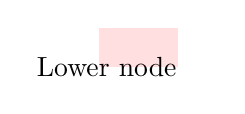
\begin{tikzpicture}[fill opacity=0.85]
%        \draw [color=gray]  [step=1mm] (0,0) grid (2,2);
%        \draw [fill=white!20] (0,0) rectangle (3.4,-.2);
%        \draw [fill=blue!20] (0,0) rectangle (3.4,-.2);
    \fill[red] (0,0) rectangle (1,0.5); 
    \fill[white] (0.0,0) rectangle (1.5,0.5);
%    \fill[blue] (0.5,0.5) rectangle (1.5,0.5);
    \node[text opacity=1] at (0.1,0) {Lower node};

%        \node at (0.2,0.2) {\sf 
%          {\tiny
%            \shortstack[c]{Select named nodes\\in reader properties}
%          }
%        };
      \end{tikzpicture}
    }
  \end{overpic}
  \caption{Generating a threshold based selection on named nodes.}
  \label{fig:pv_named_nodes_thresh_sel}
\end{figure}%

\newpage
\subsection{GMV}

\begin{figure}[htb] 
  \centering
  \begin{overpic}[grid,tics=10,width=0.5\textwidth]{pics/gmv}
    \put(10,20){\textcolor{white}{\bf The electrostatic man!}}
  \end{overpic}
  \caption{Postprocessing with General Mesh Viewer (GMV)}
  \label{fig:gmv}
\end{figure}%

\noindent File $\rightarrow$ Read GMV File  $\rightarrow$ New Simulation

\noindent Display $\rightarrow$ Cells $\rightarrow$ Select $\rightarrow$ Select On Materials and Flags $\rightarrow$ Man  $\rightarrow$ Apply

\noindent Cells dialogue  $\rightarrow$ Color By: $\rightarrow$ Node Field  $\rightarrow$ Cells dialogue: Apply

\noindent Cells dialogue  $\rightarrow$ Shaded $\rightarrow$ Apply

\noindent Menu: Calculate $\rightarrow$ Cutplanes $\rightarrow$ 1 NONE $\rightarrow$ (1,0,-0.3), (0,1,-0.3), (0,0,-0.3) $\rightarrow$ Add

\section{General}
